\documentclass[11pt]{article}
\usepackage{../../latex/preamble}

\begin{document}
  % make title page
\begin{titlepage}
  \newcommand{\HRule}{\rule{\linewidth}{0.5mm}}
  \center
  \textsc{\LARGE Universitetet i Oslo}\\[1.5cm] % Name of your university/college
  \textsc{\Large }\\[0.5cm] % Major heading such as course name
  \textsc{\large FYS3150}\\[0.5cm] % Minor heading such as course title
  \HRule \\[0.4cm]
  { \huge \bfseries En sammenligning av numeriske integrasjonsmetoder,
    Gauss kvadratur og Monte Carlo}\\[0.4cm]
  \HRule \\[1.5cm]
  \Large \emph{Skrevet av:}\\
  Lyder \textsc{Rumohr Blingsmo} og Bendik \textsc{Samseth}\\[3cm]
  {\large \today}\\[3cm]
  \vfill
\end{titlepage}

\begin{abstract}
  I denne rapporten har vi beregnet forventingsverdien til korrelasjonsenergien
  mellom to elektroner i bane rundt en heliumkjerne. Beregningen
  innebærer å løse et 6-dimensjonalt integral. Vi bruker
  Gauss-Legendre- og Gauss-Laguerre-kvadratur, samt
  Monte Carlo-integrasjon med og uten ``importance sampling''. Vi
  konkluderer med at Gauss-Legendre og standard Monte Carlo brukt
  blindt på problemstillingen fungerer mindre bra, men med litt
  tenkearbeid får vi gode resultater med Gauss-Laguerre og Monte Carlo
  med ``importance sampling''.  
\end{abstract}

\section{Innledning}
\label{sec:innledning}

Vi antar at bølgefunksjonen til hvert elektron kan skrives som en ett-partikkel
bølgefunksjon for et elektron i et hydrogenatom. Single-particle bølgefunksjonen for 
grunntilstanden er da gitt ved en dimensjonsløs variabel
\[
   {\bf r}_i =  x_i {\bf e}_x + y_i {\bf e}_y +z_i {\bf e}_z ,
\]
as
\[
   \psi_{1s}({\bf r}_i)  =   e^{-\alpha r_i},
\]
Her er ikke $\psi_{1s}$ normalisert. $\alpha$ er en parameter og
\[
r_i = \sqrt{x_i^2+y_i^2+z_i^2}.
\]
Vi setter $\alpha=2$, som tilsvarer ladningen til et heliumatom $Z=2$. 

Antar videre at bølgefunksjonen for to elektroner da kan skrives som et produkt av
to $1s$ bølgefunksjoner:
\[
   \Psi({\bf r}_1,{\bf r}_2)  =   e^{-\alpha (r_1+r_2)}.
\]

Integralet vi skal løse er den kvantemekaniske forventningsverdien
til korrelasjonsenergien til to elektroner som frastøter hverandre via et Coulumb-potensial
\begin{equation}\label{eq:correlationenergy}
   \langle \frac{1}{|{\bf r}_1-{\bf r}_2|} \rangle =
   \int_{-\infty}^{\infty} d{\bf r}_1d{\bf r}_2  e^{-2\alpha (r_1+r_2)}\frac{1}{|{\bf r}_1-{\bf r}_2|}.
\end{equation}

Her vet vi at integralet \eqref{eq:correlationenergy} har eksakt løsning $5\pi^2/16^2$. Vi skal tilnærme denne 
løsningen på fire forskjellige måter og sammenligne resultatene både i presisjon og kjøretid.

\section{Metoder}
\label{sec:metoder}
Vi anvender to forskjellige metoder for Gauss-kvadratur og to forskjellige MC-metoder.
\subsection{Gauss-kvadratur}
\label{subsec:gauss-kvadratur}
Gauss-kvadratur baserer seg på å tilnærme funksjonen vi ønsker å
integrere ved ortogonale polynomer. Teorien bak metoden er beskrevet
i~\cite{Lecture-notes}, men er litt for inngående til at det er
hensiktsmessig å gå gjennom den i denne rapporten. Det viktige er at
vi benytter et spesielt sett med polynomer; her bruker vi Legendre- og
Laguerre-polynomer. Avhengig av integralet som skal løses vil det være
hensiktsmessig å benytte et passende sett med polynomer.

\subsubsection{Rett fram med Legendre-polynomer}
\label{subsubsec:gauss-legendre}
Legendre-polynomer er definert for $x\in[-1,1]$. For å bruke disse
polynomene begynner vi med å skrive om \eqref{eq:correlationenergy} på formen

\begin{align}\label{eq:xyzINT} 
  \langle \frac{1}{|{\bf r}_1-{\bf r}_2|} \rangle =
   \int_{-\infty}^{\infty} \dots \int_{-\infty}^{\infty}
   \frac{d{x}_1d{x}_2d{y}_1d{y}_2d{z}_1d{z}_2  
   e^{-2\alpha (x_1^2+x_2^2+y_1^2+y_2^2+z_1^2+z_2^2)}}{ \sqrt{{(x_1-x_2)}^2+{(y_1-y_2)}^2+{(y_1-y_2)}^2}}
\end{align}

Her ligger $x1$, $x2$, $y1$, $y2$, $z1$ og $z2$ på intervallet 
$[-\infty, \infty]$. Dette er åpenbart umulig å representere numerisk
og vi må derfor velge et intervall $[a,b]$ som vi mapper med Legendre-polynomer.
Mer om disse polynomene står i~\cite{Lecture-notes}. I vårt tilfelle
har vi valgt intervallet $[-2,2]$ etter vurderinger av figur \ref{fig:PSI}.

\begin{figure}[ht]
  \centering
  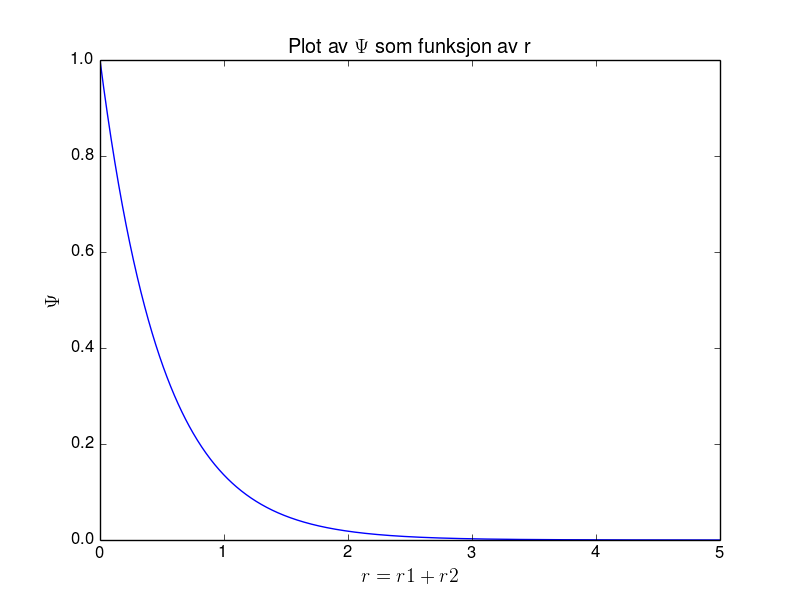
\includegraphics[scale=0.7]{../fig/psiPlot.png}
  \caption{\label{fig:PSI} Et plot av  $e^{-2\alpha (r_1+r_2)}$. Vi må velge
et intervall $[a,b]$ slik at vi får med hovedtrekkene. Vi har valgt 
intervallet $[-2,2]$. Siden vi ikke kan velge antall punkter, N,
alt for stort, må vi også ta hensyn til dette i valget av intervall.}
\end{figure}


\subsubsection{Koordinatskift og Laguerre-polynomer}
\label{susubsec:gauss-laguerre}
Laguerre-polynomene er definert for $x\in[0,\infty)$. Her begynner vi med å gjøre et koordinatskifte av 
\eqref{eq:correlationenergy} til sfæriske koordinater. Vi får da variablene

\[
   d{\bf r}_1d{\bf r}_2  = r_1^2dr_1 r_2^2dr_2 dcos(\theta_1)dcos(\theta_2)d\phi_1d\phi_2,
\]
og
\[
   \frac{1}{r_{12}}= \frac{1}{\sqrt{r_1^2+r_2^2-2r_1r_2cos(\beta)}}
\]
med 
\[
cos(\beta) = cos(\theta_1)cos(\theta_2)+sin(\theta_1)sin(\theta_2)cos(\phi_1-\phi_2))
\]

Det resulterende integralet blir

\begin{align}
\int_{0}^{\infty} r_1^2 dr_1 \int_{0}^{\infty} r_2^2 dr_2
\int_{0}^{\pi} dcos(\theta_1) \int_{0}^{\pi} dcos(\theta_2)
\int_{0}^{2\pi} d\phi_1 \int_{0}^{2\pi} d\phi_2 \frac{e^{-2\alpha (r_1+r_2)}}{r_{12}}\label{eq:int-spherical}
\end{align}

med

\[
dcos(\theta_1) = -sin(\theta_1)d\theta
\]

Her mapper vi $\phi_1$, $\phi_2$ $\theta_1$ og $\theta_2$ med
Legendre-polynomer slik som i sted (fordi $\phi\in[0,2\pi]$ og
$\theta\in[0,\pi]$ lett kan dannes fra intervallet $[-1,1]$).
Men $ r_i \in [0, \infty] $ mapper vi med
Laguerre-polynomer~\cite{Lecture-notes}. Ved å bruke disse polynomene
kan vi unngå problematikken knyttet til et intervall som går til $\infty$.


\subsection{Monte Carlo}
\label{subsec:monte-carlo}
Monte Carlo-metoder baserer seg på å velge integrasjonspunktene som
tilfeldige tall trukket fra en gitt sannsynlighetsfordeling. Tanken er
her da at bare vi inkluderer mange nok bidrag (trekker mange
tilfeldige integrasjonspunkter) så får hele integranden bidratt på en
passende måte til integralet. Tankearbeidet her legges i hovedsak inn
i hvilken sannsynlighetsfordeling man bruker.

\subsubsection{Brute force Monte Carlo}
\label{subsubsec:monte-carlo-uniform}
Vi begynner med å gå rett frem og bruke en uniform
sannsynlighetsfordeling, $p(x) = 1$. Nok en gang bruker vi
\eqref{eq:xyzINT} som utgangspunkt. Vi velger seks koordinater ($x1$,
$x2$, $y1$, $y2$, $z1$ og $z2$) uniformt fordelt og tilfeldig i
intervallet $[a,b]$. Vi velger intervallet $[-2,2]$ med samme grunnlag
som i seksjon \ref{subsubsec:gauss-legendre}. Dette gjør vi $N$ ganger, og for hver gang regner
vi ut integranden og summerer alle bidragene. Til slutt deler vi på
antall punkter, dvs. ganger med bredden på intervallet. Vi håper på
at vi ved å velge tilfeldige punkter skal klare å fange opp
oppførselen til funksjonen tilstrekkelig godt.

\subsubsection{Importance sampling Monte Carlo}
\label{susubsec:monte-carlo-importance-sampling}
Nå skal vi forsøke oss med en litt smartere valgt
sannsynlighetsfordeling. Vi tar utgangspunkt i
(\ref{eq:int-spherical}). Analogt til hvordan vi gjorde det i
\ref{susubsec:gauss-laguerre} så lar vi $\phi_1,\phi_2,\theta_1$ og
$\theta_2$ bli trukket med en uniform fordeling.

Posisjonskoordinatene skal vi derimot tenke litt mer på. Fra figur
\ref{fig:PSI} ser vi at store verdier av $r_i$ ikke vil ha store
bidrag på grunn av eksponentialet. Det virker dermed som en god idé å
trekke koordinatene $r_1,r_2$ fra en eksponentialfordeling,
\begin{align}
  p(x) = e^{-x},\hspace{0.5cm}\int_0^\infty p(x)\,dx=1.\label{eq:exponential-prob}
\end{align}
Praktisk oppnår vi dette ved følgende transformasjon:
\begin{align}
  r_i = -\ln \left( 1-x \right)
\end{align}
der $x\in[0,1]$ er trukket fra en uniform fordeling.


\section{Resultater}



\section{Konklusjon}



\printbibliography
\end{document}
%%% Local Variables:
%%% mode: latex
%%% TeX-master: t
%%% End:
